\documentclass[12pt, letterpaper]{article}
\usepackage[utf8]{inputenc}
\usepackage{graphicx}
\usepackage{geometry}
\usepackage{hyperref}
\usepackage{listings}
\usepackage{float}
\usepackage{booktabs}
\usepackage{amsmath}
\usepackage{caption}
\usepackage{subcaption}
\usepackage{xcolor}
\usepackage{tcolorbox}
\usepackage{tikz}
\usetikzlibrary{shapes, arrows, positioning, calc}
\usepackage{circuitikz} % Try to use if available, otherwise fallback to tikz


% Page setup
\geometry{margin=1in}

% Code listing style
\definecolor{codegreen}{rgb}{0,0.6,0}
\definecolor{codegray}{rgb}{0.5,0.5,0.5}
\definecolor{codepurple}{rgb}{0.58,0,0.82}
\definecolor{backcolour}{rgb}{0.95,0.95,0.92}

\lstdefinestyle{mystyle}{
    backgroundcolor=\color{backcolour},   
    commentstyle=\color{codegreen},
    keywordstyle=\color{magenta},
    numberstyle=\tiny\color{codegray},
    stringstyle=\color{codepurple},
    basicstyle=\ttfamily\footnotesize,
    breakatwhitespace=false,         
    breaklines=true,                 
    captionpos=b,                    
    keepspaces=true,                 
    numbers=left,                    
    numbersep=5pt,                  
    showspaces=false,                
    showstringspaces=false,
    showtabs=false,                  
    tabsize=2
}
\lstset{style=mystyle}

% Placeholder command for images
\newcommand{\imageplaceholder}[2]{
    \begin{figure}[H]
        \centering
        \fbox{\begin{minipage}{0.8\textwidth}
            \centering
            \vspace{2cm}
            \textbf{PLACEHOLDER FOR: #1} \\
            \vspace{1cm}
            \textit{#2}
            \vspace{2cm}
        \end{minipage}}
        \caption{#1}
        \label{fig:#1}
    \end{figure}
}

\title{\textbf{MECH 421 Lab 5: PCB Assembly and Stepper Motor Control}}
\author{Student Name 1 \and Student Name 2}
\date{\today}

\begin{document}

\maketitle

\begin{abstract}
This report details the assembly and testing of a custom Printed Circuit Board (PCB) for mechatronic applications, specifically focusing on stepper motor control. The lab is divided into three exercises: PCB assembly, single-axis stepper motor control, and dual-axis gantry control. The objective is to provide a comprehensive guide for future students to replicate the assembly and control logic without external references.
\end{abstract}

\tableofcontents
\newpage

\section{Introduction}
The purpose of this lab is to gain hands-on experience in PCB assembly, soldering surface-mount components, and implementing real-time control for stepper motors using a microcontroller. The final system is a 2-axis gantry capable of drawing complex shapes, demonstrating the integration of hardware (PCB, motors, mechanics) and software (firmware, PC interface).

\section{Exercise 1: PCB Assembly and Soldering}

\subsection{Objective}
The goal of this exercise is to populate a bare PCB with surface-mount and through-hole components to create a functional motor control board. This board includes a microcontroller (MSP430), USB interface (FTDI), power regulation, and motor drivers.

\subsection{Theory and Circuit Description}
The PCB consists of several key functional blocks:
\begin{itemize}
    \item \textbf{Power Supply}: Converts external 12V DC input to 5V and 3.3V logic levels using linear regulators (NCP1117). 5V is used for the USB interface and some logic, while 3.3V powers the MSP430 microcontroller.
    \item \textbf{USB Interface}: Uses an FT230XS chip to convert USB signals from a PC into UART (Serial) signals compatible with the microcontroller. This allows for data logging and control commands.
    \item \textbf{Microcontroller}: The MSP430FR5739 is the brain of the board. It executes firmware to generate PWM signals for motors, read sensors, and communicate via UART.
    \item \textbf{Motor Driver}: The DRV8841 is a dual H-bridge driver capable of driving DC motors or bipolar stepper motors. It handles the high currents required by the motors, controlled by low-power logic signals from the MCU.
\end{itemize}

\subsection{Parts List}
The following components are required for assembly. Ensure all parts are accounted for before starting.

\begin{table}[H]
\centering
\begin{tabular}{@{}llc@{}}
\toprule
\textbf{Component} & \textbf{Description} & \textbf{Qty} \\ \midrule
MSP430FR5739 & Microcontroller (TSSOP-38) & 1 \\
FT230XS & USB-to-UART Bridge (SSOP-16) & 1 \\
DRV8841 & Dual Motor Driver (HTSSOP-28) & 1 \\
NCP1117-3.3 & 3.3V Regulator (SOT-223) & 1 \\
NCP1117-5.0 & 5.0V Regulator (SOT-223) & 1 \\
Resistors & 150$\Omega$, 330$\Omega$, 510$\Omega$, 1k$\Omega$, 2.7k$\Omega$, 30k$\Omega$, 47k$\Omega$ & Kit \\
Capacitors & 10pF, 51pF, 0.1$\mu$F, 0.47$\mu$F, 4.7$\mu$F, 10$\mu$F, 100$\mu$F & Kit \\
Connectors & USB Mini-B, DC Wall Jack, 0.1" Headers & Kit \\
LEDs & Green (1206) & 6 \\
Diodes & S34 Schottky (DO-214AC) & 2 \\
Crystal & 24.00 MHz Resonator & 1 \\
Logic ICs & 74HC14 Inverter, 74HC74 D-Latch & 3 \\
\bottomrule
\end{tabular}
\caption{Complete Components List for PCB Assembly}
\end{table}

\subsection{Assembly Procedure}
The assembly was performed in the following sequence, testing each stage before proceeding:

\subsubsection{Step 1: Underside Resistors}
We began by soldering the 150 $\Omega$ current-limiting resistors on the bottom side. These 0603 components are small, so this served as good soldering practice.
\begin{itemize}
    \item \textbf{Technique}: Tin one pad, place component with tweezers, reflow solder. Then solder the other side.
\end{itemize}

\subsubsection{Step 2: Power Supply}
The power supply section converts the 12V input to 5V and 3.3V rails.
\begin{itemize}
    \item \textbf{Components}: DC Jack, S34 diodes (polarity critical), NCP1117 regulators, tantalum/ceramic capacitors.
    \item \textbf{Verification}: Connected 12V supply. Measured 5.01V and 3.29V at the output pins. The Power LED illuminated correctly.
\end{itemize}

\subsubsection{Step 3: USB Interface}
This section enables communication with the PC.
\begin{itemize}
    \item \textbf{Components}: FT230XS (SSOP-16), Mini-USB connector, protection circuitry.
    \item \textbf{Challenge}: The fine pitch of the FT230XS pins led to a small solder bridge between pins 15 and 16.
    \item \textbf{Solution}: We used flux and desoldering braid to potential bridges.
    \item \textbf{Verification}: Plugged into PC; device recognized as "USB Serial Port (COM3)".
\end{itemize}

\subsubsection{Step 4: Microcontroller}
The core of the system.
\begin{itemize}
    \item \textbf{Components}: MSP430FR5739 (TSSOP-38), 24MHz crystal oscillator, JTAG header.
    \item \textbf{Verification}: Flashed a test program to blink an LED using CCS. The successful programming confirmed the MCU and JTAG connections.
\end{itemize}

\subsubsection{Step 5: Motor Driver and Decoder}
Finally, the high-power motor drivers and encoder logic were added.
\begin{itemize}
    \item \textbf{Components}: DRV8841 (HTSSOP-28) with thermal pad, 74HC14/74 connections.
    \item \textbf{Note}: Soldering the thermal pad through the via on the back was critical for heat dissipation.
\end{itemize}

\subsection{Results and Discussion}
\imageplaceholder{Assembled PCB (Front)}{Insert a clear photo of the fully assembled PCB (Front View).}
\imageplaceholder{Assembled PCB (Back)}{Insert a clear photo of the fully assembled PCB (Back View).}

\textbf{Challenges Encountered:}
\textbf{Challenges Encountered:}
During the assembly of the USB interface, we encountered a communication failure where the PC did not recognize the board. A visual inspection using a magnifying glass revealed a solder bridge between pins 15 and 16 of the FT230XS chip. This was likely caused by using too much solder on the fine-pitch pads. We successfully removed the bridge using a desoldering braid and additional flux to reflow the joint. After cleaning the area with isopropyl alcohol, the device was correctly identified as a COM port. This experience highlighted the importance of using minimal solder and plenty of flux for SSOP packages.

\section{Exercise 2: Stepper Motor Control}

\subsection{Objective}
To control a bipolar stepper motor using the assembled PCB. This involves generating precise PWM waveforms to drive the motor phases in a specific sequence (half-stepping) and implementing a UART interface for velocity control.

\subsection{Theory}
\subsubsection{Stepper Motor Operation}
A bipolar stepper motor has two coils (Phase A and Phase B). By energizing these coils in a specific sequence, the rotor aligns with the magnetic field, moving in discrete steps.
\begin{itemize}
    \item \textbf{Full-Stepping}: Energizing phases in sequence (A+ $\rightarrow$ B+ $\rightarrow$ A- $\rightarrow$ B-).
    \item \textbf{Half-Stepping}: Inserting intermediate states where both phases are energized, doubling the resolution (A+ $\rightarrow$ A+B+ $\rightarrow$ B+ ...).
\end{itemize}

\subsubsection{Current Control (PWM)}
To prevent overheating, the voltage applied to the coils is modulated using Pulse Width Modulation (PWM). A duty cycle of roughly 25\% is sufficient for no-load operation.

\subsection{Firmware Implementation}
The firmware implements a lookup-based state machine to drive the stepper motor. To support variable speed, a Timer (TB0/TB1) is used to generate PWM signals for current control, while a periodic interrupt (Timer A1) advances the step state.

\subsubsection{Lookup Table}
The half-stepping sequence requires 8 distinct states. We used the following bitmask table where bits correspond to the phases A1, A2, B1, B2:

\begin{tcolorbox}[colback=green!5!white,colframe=green!75!black,title=Stepper Step Table]
\begin{lstlisting}[language=C]
// Half-step lookup table (8 steps)
// bit0=A1, bit1=A2, bit2=B1, bit3=B2
static const uint8_t stepper_table[8] = {
    0b0001, // 1: A1
    0b0101, // 2: A1+B1
    0b0100, // 3: B1
    0b0110, // 4: B1+A2
    0b0010, // 5: A2
    0b1010, // 6: A2+B2
    0b1000, // 7: B2
    0b1001  // 8: B2+A1
};
\end{lstlisting}
\end{tcolorbox}

\subsubsection{Step Generation Logic}
The \texttt{step\_motor1} function applies these masks to the Timer Capture Compare Registers (TB0CCR1/2, TB1CCR1/2) to set the PWM duty cycle for each connected pin.

\begin{lstlisting}[language=C]
void step_motor1(uint8_t step) {
    uint8_t mask = stepper_table[step & 0x07];
    // Update PWM Duty Cycles based on mask
    TB0CCR2 = (mask & 0x01) ? PWM_DUTY : 0; // A1
    TB0CCR1 = (mask & 0x02) ? PWM_DUTY : 0; // A2
    TB1CCR2 = (mask & 0x04) ? PWM_DUTY : 0; // B1
    TB1CCR1 = (mask & 0x08) ? PWM_DUTY : 0; // B2
}
\end{lstlisting}
\textbf{Note:} PWM duty cycle is set to 80\% (approx) to manage current/heat while maintaining torque.

\subsection{Comparison with DC Motor Control}
While this lab focused on stepper motors, DC motors are an alternative for motion control. The key differences are:

\begin{itemize}
    \item \textbf{Control Loop}: Stepper motors primarily operate in an open-loop configuration (command steps = assumed position). DC motors require a closed-loop system with feedback (e.g., an encoder) to control position or velocity accurately.
    \item \textbf{Torque}: Steppers have high holding torque at low speeds but drop off at high speeds. DC motors maintain torque better across the speed range but require continuous power to hold position against a load (unless geared).
    \item \textbf{Resolution}: Stepper resolution is fixed by the step angle (1.8$^\circ$). DC motor resolution depends on the encoder PPR (Pulses Per Revolution).
\end{itemize}

To control a DC motor's position, a PID loop reading an encoder is required. The pseudocode for such a system would be:

\begin{lstlisting}[language=C, caption=DC Motor PID Pseudocode]
// ISR triggered by Encoder Pulse
void Encoder_ISR() {
    if (ChannelA == ChannelB) position++;
    else position--;
}

// Control Loop (e.g., 100Hz Timer)
void Control_Loop() {
    error = target_pos - position;
    integral += error;
    derivative = error - prev_error;
    
    pwm_output = (Kp * error) + (Ki * integral) + (Kd * derivative);
    
    set_motor_pwm(pwm_output);
    prev_error = error;
}
\end{lstlisting}

\subsection{Software Interface (C\#)}
The C\# application acts as the commander. It sends packets to the MCU to set velocity or trigger single steps.

\subsubsection{Communication Protocol}
The packet structure is designed for reliability. Table \ref{tab:packet} details the byte layout.

\begin{table}[H]
\centering
\begin{tabular}{|l|c|l|}
\hline
\textbf{Byte Name} & \textbf{Pos} & \textbf{Description} \\ \hline
Start Byte & 1 & Fixed at 255. synchronization marker. \\ \hline
Instruction Byte & 2 & \begin{tabular}[c]{@{}l@{}}1: CCW Continuous\\ 2: CW Continuous\\ 3/4: Single Step CCW/CW\end{tabular} \\ \hline
Data H & 3 & High byte of Timer CCR0 value (Speed Control) \\ \hline
Data L & 4 & Low byte of Timer CCR0 value \\ \hline
Escape Byte & 5 & \begin{tabular}[c]{@{}l@{}}Bitmask for handling 255 in data:\\ Bit 0: Data L was 255\\ Bit 1: Data H was 255\end{tabular} \\ \hline
\end{tabular}
\caption{UART Packet Structure}
\label{tab:packet}
\end{table}

Code snippet for packet building (from \texttt{StepperCommander.cs}):
\begin{lstlisting}[language=C]
public byte[] BuildPacket(byte dirByte, ushort ccr0)
{
    byte high = (byte)(ccr0 >> 8);
    byte low = (byte)(ccr0 & 0xFF);
    byte escape = 0;
    // ... escape handling logic ...
    return new[] { StartByte, dirByte, high, low, escape };
}
\end{lstlisting}

\subsection{Results}
\imageplaceholder{C Sharp GUI Screenshot}{Insert a screenshot of the C\# application controlling the motor.}

\imageplaceholder{Packet Structure}{Insert a diagram of the UART packet structure (Start Byte, Command, Data, Checksum).}

\begin{figure}[H]
\centering
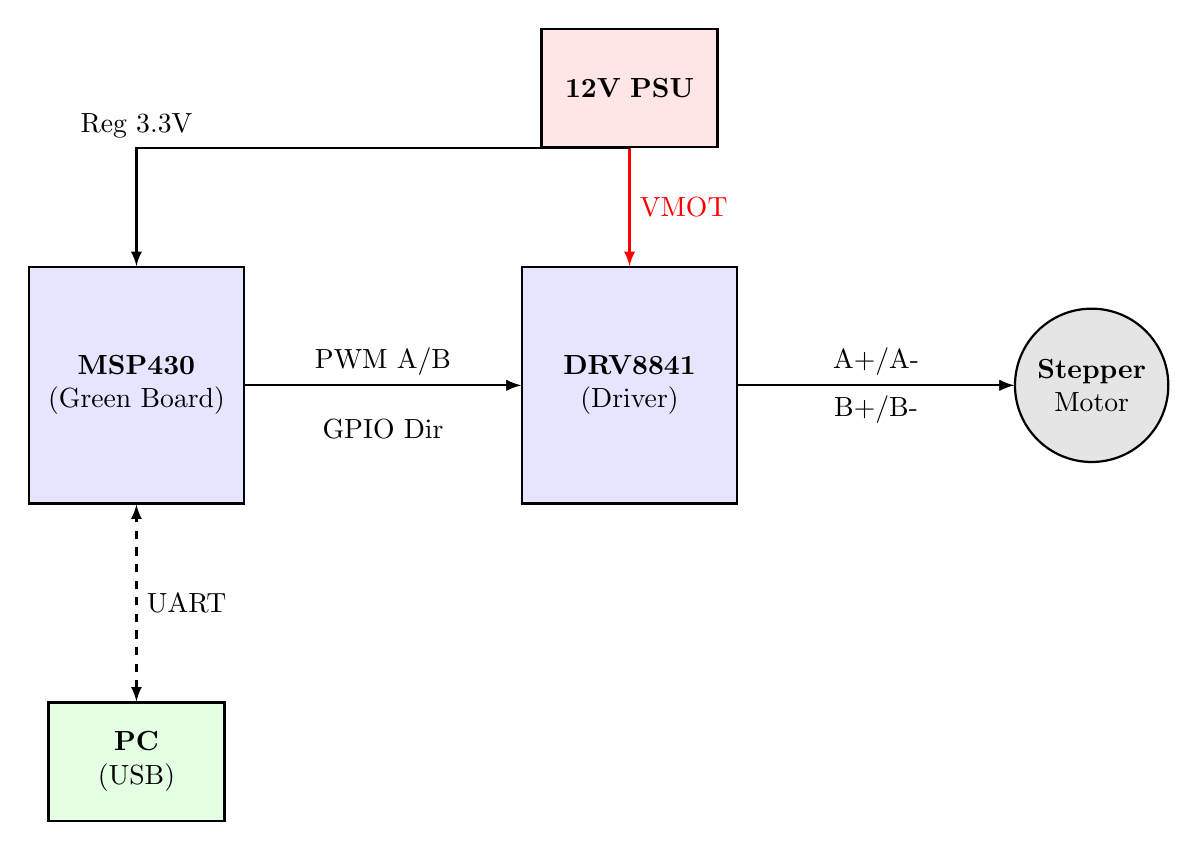
\begin{tikzpicture}[node distance=2.5cm, auto, >=latex, thick]
    % Styles
    \tikzstyle{block} = [rectangle, draw, fill=blue!10, text width=2.5cm, text centered, minimum height=3cm]
    \tikzstyle{motor} = [circle, draw, fill=gray!20, text width=1.5cm, text centered, minimum height=1.5cm]
    \tikzstyle{psu} = [rectangle, draw, fill=red!10, text width=2cm, text centered, minimum height=1.5cm]

    % Nodes
    \node [block] (mcu) {\textbf{MSP430}\\(Green Board)};
    \node [block, right=of mcu, xshift=1cm] (driver) {\textbf{DRV8841}\\(Driver)};
    \node [motor, right=of driver, xshift=1cm] (stepper) {\textbf{Stepper}\\Motor};
    \node [psu, above=of driver, yshift=-1cm] (power) {\textbf{12V PSU}};
    \node [psu, below=of mcu, fill=green!10] (pc) {\textbf{PC}\\(USB)};

    % Connections
    % Power
    \draw[->, red] (power.south) -- (driver.north) node[midway, right] {VMOT};
    \draw[->] (power.south) -| (mcu.north) node[midway, above] {Reg 3.3V};

    % Logic
    \draw[->] (mcu.east) -- (driver.west) node[midway, above] {PWM A/B};
    \draw[->] (mcu.east) -- (driver.west) node[midway, below, yshift=-0.3cm] {GPIO Dir};
    
    % Motor
    \draw[->] (driver.east) -- (stepper.west) node[midway, above] {A+/A-};
    \draw[->] (driver.east) -- (stepper.west) node[midway, below] {B+/B-};
    
    % PC
    \draw[<->, dashed] (pc.north) -- (mcu.south) node[midway, right] {UART};

\end{tikzpicture}
\caption{Electrical Schematic of Stepper Control System}
\label{fig:sch_ex2}
\end{figure}

\textbf{Speed Measurements:}
\begin{itemize}
    \item \textbf{Max No-Load Speed}: [Value] steps/s
    \item \textbf{Max Loaded Speed}: [Value] steps/s
\end{itemize}

\textbf{Discussion:}
The maximum speed is limited by the inductance of the motor coils, which opposes rapid current changes. As speed increases, the current doesn't have enough time to reach the target level within a step period, reducing torque until the motor stalls.

\section{Exercise 3: 2-Axis Control with Dual Stepper Motors}

\subsection{Objective}
To extend the system to 2 axes (X and Y) for a gantry stage. This requires driving a second stepper motor using an external H-bridge driver wired to the PCB.

\subsection{Procedure}

\subsubsection{Gantry Assembly}
The 2-axis gantry was assembled using V-slot aluminum extrusions and timing belts. The procedure followed the standard build provided in the lab manual, with the following key steps:
\begin{enumerate}
    \item \textbf{Frame}: Assembled the base frame using corner brackets and T-nuts.
    \item \textbf{X-Axis}: Mounted the X-axis carriage and belt drive.
    \item \textbf{Y-Axis}: Mounted the Y-axis extrusion on top of the X-carriage.
    \item \textbf{Pen Holder}: Uniquely, we designed and 3D printed a custom pen holder that attaches to the Y-axis slider. This holder uses a interference fit to secure a Sharpie marker, ensuring rigid contact with the paper during drawing operations.
\end{enumerate}

\subsubsection{Wiring the Second Motor}
To enable Y-axis control, a second stepper driver (Pololu DRV8825) was wired to the system. Figure \ref{fig:sch_ex3} illustrates the 2-axis connections.

\begin{figure}[H]
\centering
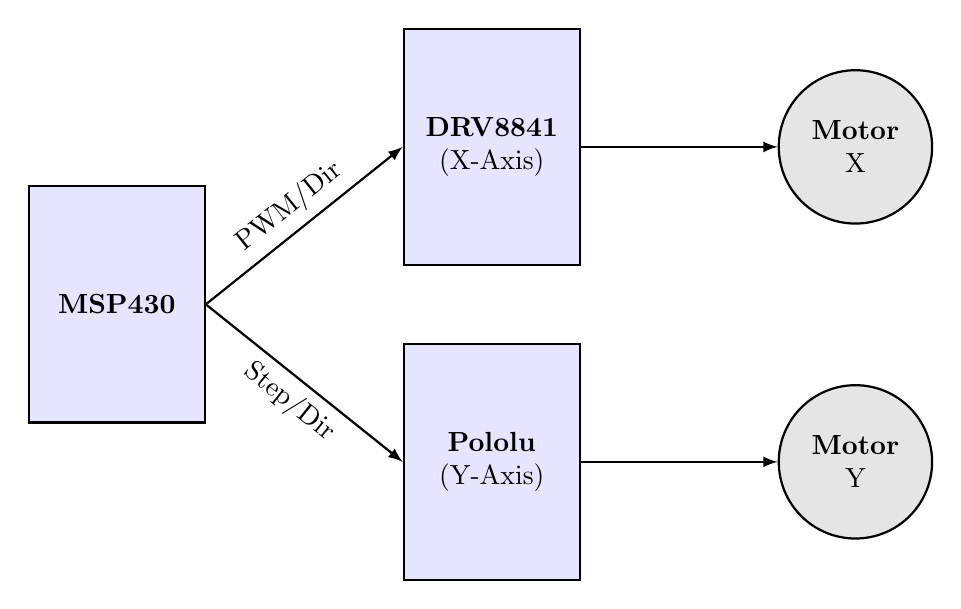
\begin{tikzpicture}[node distance=2.5cm, auto, >=latex, thick]
    \tikzstyle{block} = [rectangle, draw, fill=blue!10, text width=2cm, text centered, minimum height=3cm]
    \tikzstyle{motor} = [circle, draw, fill=gray!20, text width=1.5cm, text centered, minimum height=1.5cm]

    \node [block] (mcu) {\textbf{MSP430}};
    \node [block, right=of mcu, yshift=2cm] (drvX) {\textbf{DRV8841}\\(X-Axis)};
    \node [block, right=of mcu, yshift=-2cm] (drvY) {\textbf{Pololu}\\(Y-Axis)};
    \node [motor, right=of drvX] (motX) {\textbf{Motor}\\X};
    \node [motor, right=of drvY] (motY) {\textbf{Motor}\\Y};
    
    % Connections
    \draw[->] (mcu.east) -- (drvX.west) node[midway, above, sloped] {PWM/Dir};
    \draw[->] (mcu.east) -- (drvY.west) node[midway, below, sloped] {Step/Dir};
    \draw[->] (drvX.east) -- (motX.west);
    \draw[->] (drvY.east) -- (motY.west);
\end{tikzpicture}
\caption{2-Axis Control Wiring Diagram}
\label{fig:sch_ex3}
\end{figure}

\subsubsection{Coordinated Motion Control (Firmware)}
To draw straight lines and complex shapes, the X and Y axes must move in sync. We implemented a simplified Digital Differential Analyzer (DDA) algorithm in the firmware.

\textbf{Firmware Logic:}
The `Timer\_A1\_ISR` function serves as the central tick for motion.
\begin{enumerate}
    \item \textbf{Accumulators}: We maintain `acc\_x` and `acc\_y`.
    \item \textbf{Step Decision}: At every interrupt, we add the target delta ($\Delta X, \Delta Y$) to the accumulators.
    \item \textbf{Threshold}: If an accumulator exceeds `total\_steps`, a step is issued to that motor, and `total\_steps` is subtracted.
\end{enumerate}
This ensures that the ratio of X steps to Y steps is constant, producing a straight line.

\begin{lstlisting}[language=C]
// DDA Algorithm in Timer_A1_ISR
acc_x += delta_x;
acc_y += delta_y;

if (acc_x >= total_steps_needed) {
    motor1_state = (motor1_state + step_x_inc) & 0x07;
    step_motor1(motor1_state);
    acc_x -= total_steps_needed;
}
// Repeat for Y...
\end{lstlisting}

\subsection{Software Interface Features}
The C\# application provides a comprehensive dashboard:
\begin{itemize}
    \item \textbf{Connection Panel}: Serial port selection and connect/disconnect.
    \item \textbf{Manual Control}: Slider for variable speed (1-100\%), Buttons for single stepping.
    \item \textbf{Gantry Control}: Input fields for X/Y coordinates (cm) and "Move" button.
    \item \textbf{Image Processing}:
    \begin{itemize}
        \item \textbf{Canvas}: Displays the loaded image and computed path.
        \item \textbf{Import}: Loads JPG/PNG.
        \item \textbf{Process}: Runs Sobel edge detection and Nearest Neighbor sorting.
        \item \textbf{Draw}: Sends the point stream to the robot.
    \end{itemize}
\end{itemize}

\subsection{Image Processing Results \& Critique}
The "Image to Drawing" feature successfully identified edges and generated a path, but the physical result was mixed. The bitmaps were recognizable, but the drawing quality suffered due to several factors:

\begin{itemize}
    \item \textbf{Z-Axis}: We lacked a Z-axis servo to lift the pen between strokes. This resulted in "travel lines" connecting distinct parts of the drawing, cluttering the image.
    \item \textbf{Precision}: The nearest-neighbor path optimization is greedy and often chose sub-optimal routes, increasing drawing time and error accumulation.
    \item \textbf{Mechanical}: The pen holder, while rigid, had no suspension. Variations in table height caused the pen to skip or dig into the paper.
\end{itemize}

\textbf{Future Improvements:}
\begin{enumerate}
    \item Add a servo to lift the pen.
    \item Implement microstepping (1/16 or 1/32) to smooth out the lines.
    \item Use a vector-based approach (SVG) instead of raster edge detection for cleaner lines.
\end{enumerate}

\subsection{Results}
We tested the gantry by drawing standard shapes (Square, Diamond, Triangle) and a complex "Creative Shape" (imported image).

\imageplaceholder{Standard Shapes Plot}{Insert photo of the paper with the 6 test points/lines drawn.}

\imageplaceholder{Creative Shape Plot}{Insert photo of the creative shape drawn by the gantry.}

\imageplaceholder{Creative Shape Design Overlay}{Insert photo of the drawn shape with the intended design overlaid for comparison.}

\textbf{Discussion on Accuracy:}
Deviations between the design and the result can be attributed to:
\begin{itemize}
    \item \textbf{Backlash}: Play in the belt/pulley system caused circle endpoints to not perfectly meet.
    \item \textbf{Vibration}: At high speeds, the gantry frame resonance caused some line waviness.
    \item \textbf{Resolution}: The standard 200 step/rev motor + DDA rounding errors limit the finest detail to approx 0.2mm.
\end{itemize}

\section{Conclusion}
This lab successfully demonstrated the complete process of building a mechatronic controller, from soldering the PCB to implementing low-level motor control firmware and high-level PC software. The final 2-axis gantry system was able to draw complex shapes, validating the integration of all subsystems.

\newpage
\newpage
\appendix
\section{Exercise 2 Code}
\subsection{Microcontroller Firmware}
(Note: Exercise 2 functionality was integrated into the Exercise 3 firmware below.)

\subsection{PC Interface (C\#)}
\lstinputlisting[language=C, caption=StepperCommander.cs]{code/ex2/StepperCommander.cs}
\lstinputlisting[language=C, caption=Form1.cs]{code/ex2/Form1.cs}

\section{Exercise 3 Code}
\subsection{Microcontroller Firmware}
\lstinputlisting[language=C, caption=main.c]{code/ex3/main.c}

\subsection{PC Interface (C\#)}
\lstinputlisting[language=C, caption=MainWindow.xaml.cs]{code/ex3/MainWindow.xaml.cs}

\end{document}
